%%%%%%%%%%%%%%%%%%%%%%%%%%%%%%%%%%%%
% This is the template for submission to ISCA 2018
% The cls file is a modified from  'sig-alternate.cls'
%%%%%%%%%%%%%%%%%%%%%%%%%%%%%%%%%%%%

\documentclass{sig-alternate} 
\usepackage{mathptmx} % This is Times font

\newcommand{\ignore}[1]{}
\usepackage{fancyhdr}
\usepackage[normalem]{ulem}
\usepackage[hyphens]{url}
\usepackage{microtype}
\usepackage{epsfig}

% Always include hyperref last
\usepackage[bookmarks=true,breaklinks=true,letterpaper=true,colorlinks,linkcolor=black,citecolor=blue,urlcolor=black]{hyperref}

% Ensure letter paper
\pdfpagewidth=8.5in
\pdfpageheight=11in


%%%%%%%%%%%---SETME-----%%%%%%%%%%%%%
\newcommand{\iscasubmissionnumber}{NaN}
%%%%%%%%%%%%%%%%%%%%%%%%%%%%%%%%%%%%

%\fancypagestyle{firstpage}{
%  \fancyhf{}
%\renewcommand{\headrulewidth}{0pt}
%  \fancyhead[C]{\normalsize{ISCA 2018 Submission
%      \textbf{\#\iscasubmissionnumber} \\ Confidential Draft: DO NOT DISTRIBUTE}} 
%  \fancyfoot[C]{\thepage}
%}  

\pagenumbering{arabic}

%%%%%%%%%%%---SETME-----%%%%%%%%%%%%%
\title{Suitable Data Structures for Heterogeneous Memory} 
\author{Jae Woo Joo}
%%%%%%%%%%%%%%%%%%%%%%%%%%%%%%%%%%%%

\begin{document}
\maketitle
%\thispagestyle{firstpage}
\pagestyle{plain}

%\begin{abstract}

%This document is intended to serve as a sample for submissions to ISCA 2018. We provide some guidelines that authors should follow when submitting papers to the conference. In an effort to respect the efforts of reviewers and in the interest of fairness to all prospective authors, we request that all submissions follow the formatting and submission rules detailed below. 

%\end{abstract}

\section{Introduction}

Nowadays data center applications such as in-memory databases \cite{stonebraker2013voltdb} and key-value stores \cite{Redis, Memcached} require increasingly large memory capacities to handle exponentially expanding datasets, but confront the challenges due to the difficulties in scaling DRAM and the cost of DRAM. Because of the limitations, the current DRAM structure will be unsuitable in the future. In order to overcome this challenge, researchers are exploring new memory technologies such as non-volatile memory (NVM). Table 1 summarizes the key attributes of byte-addressable NVM such as phase change memory (PCM) and DRAM. NVM provides higher capacity (5$\times$) than DRAM, but lower read (2$\times$ to 4$\times$) and write (5$\times$ to 10$\times$) latency, and lower bandwidth (4$\times$ to 8$\times$) \cite{venkataraman2011consistent, dulloor2016data, kannan2017heteroos}. This implies that current memory management technology is inefficient for data center and thus future systems demand heterogeneous memory architecture by combining DRAM and NVM.

Attaching NVM and DRAM directly as NUMA nodes to the systems reusing the existing OS could be efficient in terms of the cost and scaling benefits \cite{dulloor2016data}. However, there exists a concern about the performance overheads due to the slower latency compared to the DRAM. The goal of homogeneous memory system is to maximize temporal and spatial locality when accessing data in order to reduce the latency. Compared to the homogeneous memory system, heterogeneous memory system make demands on placing appropriate data into the fastest memory. Placing the critical data in inappropriate memory could lead to a performance overhead with less than 50\% overheads \cite{kannan2017heteroos}. Therefore, taking full advantage of heterogeneous memory technologies requires changes in OS-level. 

Even though many data center applications try to optimize the data to take advantages of memory efficiency \cite{dulloor2016data}, OS kernel plays an important role in large memory systems performance such as memory allocation, page migration, and network. Thus it is crucial to understand the OS-level data structure in order to leverage the performance in heterogeneous memory systems. To gain insight into understanding the kernel data structure in OS-level, we pose the following questions: (1) What is the usage pattern and the access pattern when stressing out a specific subsystem? (2) Are current data structures suitable for heterogeneous memory systems? (3) If not, how could we make changes to the OS kernel to improve the performance?

 To answer these questions, we conduct experiments with microbenchmarks and we present the modification of the OS design which can be adapted to heterogeneous memory systems. This paper makes the following contributions:

\begin{itemize}
\item \textbf{New profiling mechanism for memory management in OS-level.} We build a tool to collect and trace the data inside the kernel to see how the kernel data structures are used for NVM.

\item  \textbf{Modification of data structures in OS-level.} We revise several kernel data structures which are commonly used in the kernel in order to improve the performance of heterogeneous memory systems. (More information needed.)

\item \textbf{Comprehensive evaluation.} We evaluate our OS design with various data center applications which concentrates on memory, storage, and network respectively. (More information needed.)
\end{itemize}
 
To the best of our knowledge, this is the first in-depth study of profiling the usage and the characteristics of various data structures in the OS-level. We conjecture that this study will benefit commercial vendors. The results of this study can help the researchers to understand and to overcome the overheads when designing the heterogeneous memory systems.

\begin{table}[t]
\centering
\begin{tabular}{|l|l|l|}
\hline
                 & DRAM       & NVM        \\ \hline
Cost             & 5$\times$        & 1$\times$        \\ \hline
Capacity per CPU & 100s of GB & Terabytes  \\ \hline
Read Latency     & 1$\times$        & 2$\times$ - 4$\times$  \\ \hline
Write Latency    & 1$\times$        & 5$\times$ - 10$\times$ \\ \hline
Bandwidth        & 4$\times$ - 8$\times$  & 1$\times$        \\ \hline
\end{tabular}
\caption{Comparison of new memory technologies \cite{venkataraman2011consistent, dulloor2016data, kannan2017heteroos}}
\end{table}

(Additional paragraph) In large memory systems, not only the data from the application but also the kernel data structures should be allocated to certain memory (e.g., DRAM, NVM). When the application has different memory access patterns, it could touch the same page multiple times or it could touch different pages. Hence, placing the kernel data structures in an appropriate place in heterogeneous memory systems is critical. We extract the information from the OS-level how kernel data structures use different memory pages. 

\section{Motivation}


\begin{figure}
  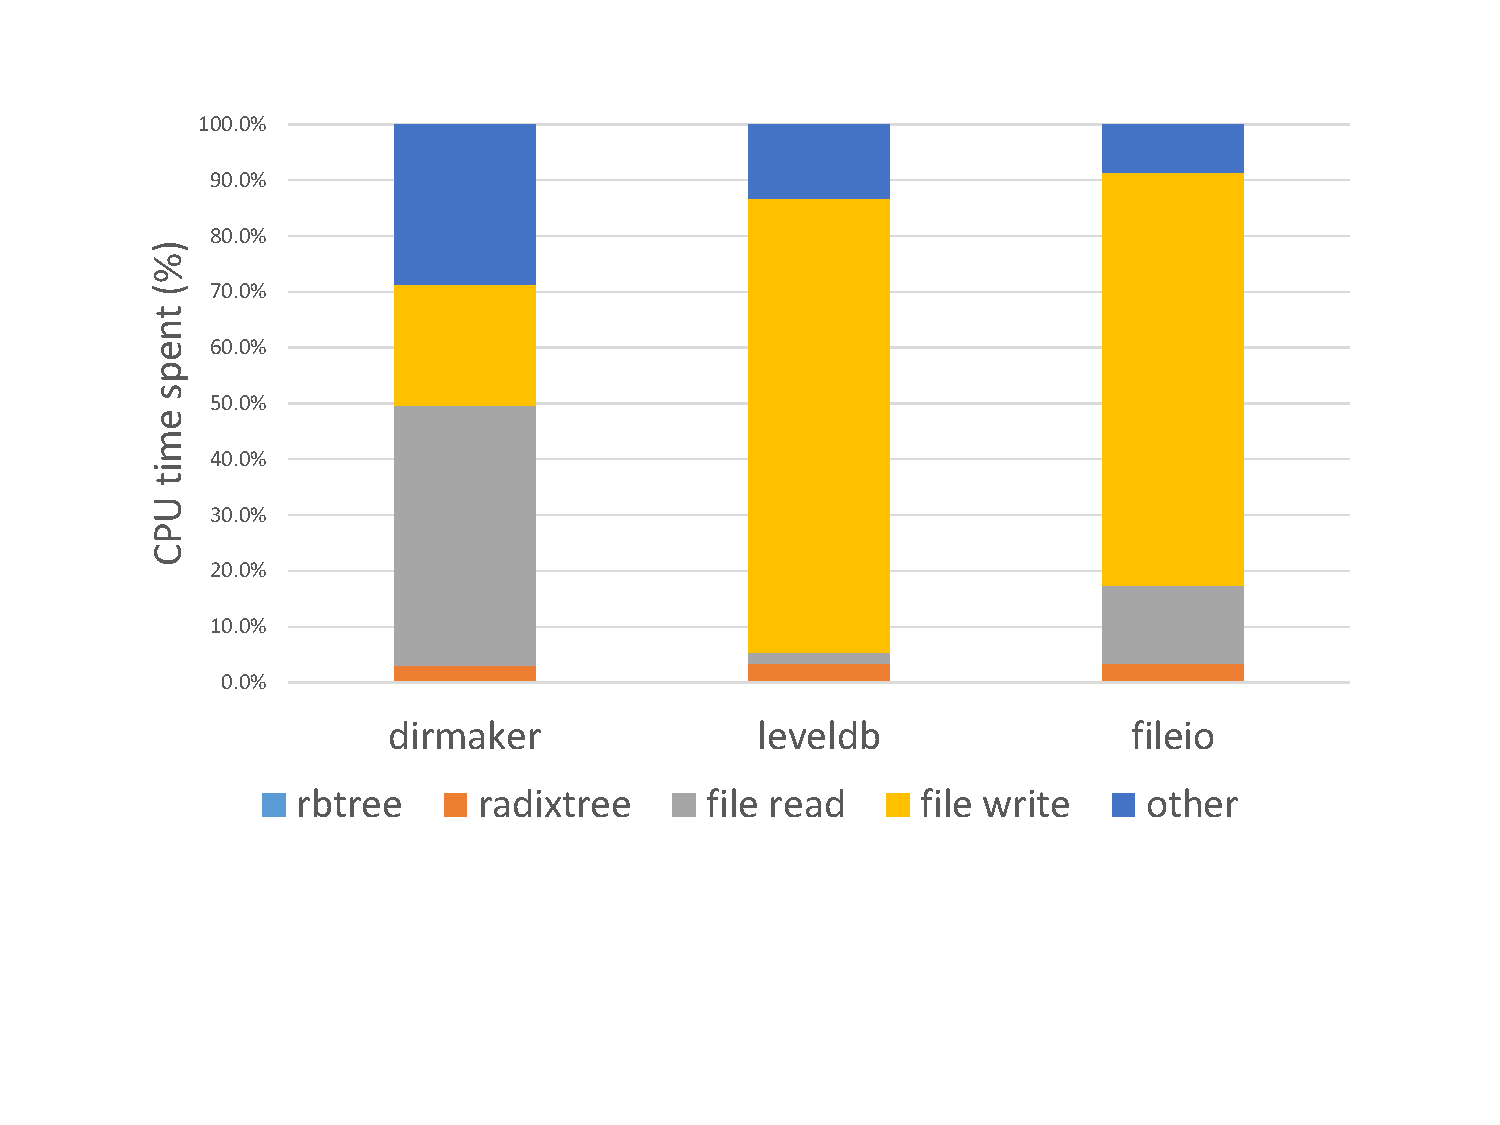
\includegraphics[width=85mm]{cputime.pdf}
  \caption{CPU time spent on major functions in applications}
  \label{cputime}
\end{figure}
\section{Related Work}
Agarwal et al. \cite{Agarwal:2015:PPS:2694344.2694381} proposed a new page placement policy that improves GPU performance in heterogeneous memory systems which differs the memory bandwidth capabilities. The proposed page placement policy places the critical data in the appropriate memory which improves the GPU performance. They use the profiling mechanism to collect the information of GPU application data structure memory access patterns and the size of the data structures allocated in the program. 


%%%%%%% -- PAPER CONTENT ENDS -- %%%%%%%%

%%%%%%%%% -- BIB STYLE AND FILE -- %%%%%%%%
\bibliographystyle{ieeetr}
\bibliography{ref}
%%%%%%%%%%%%%%%%%%%%%%%%%%%%%%%%%%%%

\end{document}
